\section{Diagramas de \textit{hardware}}

\subsection{Diagrama de Blocos}

\begin{figure}
    \centering
    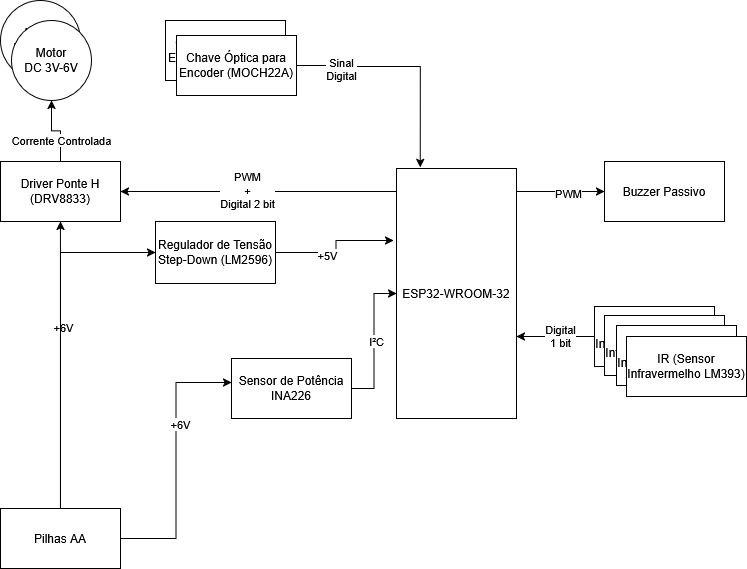
\includegraphics[width=0.5\linewidth]{figuras/diagrama_micromouse_final.drawio(1).png}
    \caption{Diagrama de blocos dos componentes eletrônicos do \textit{micromouse}}
    \label{fig:diag_hw}
\end{figure}

\subsection{Esquematico}

\begin{figure}
    \centering
    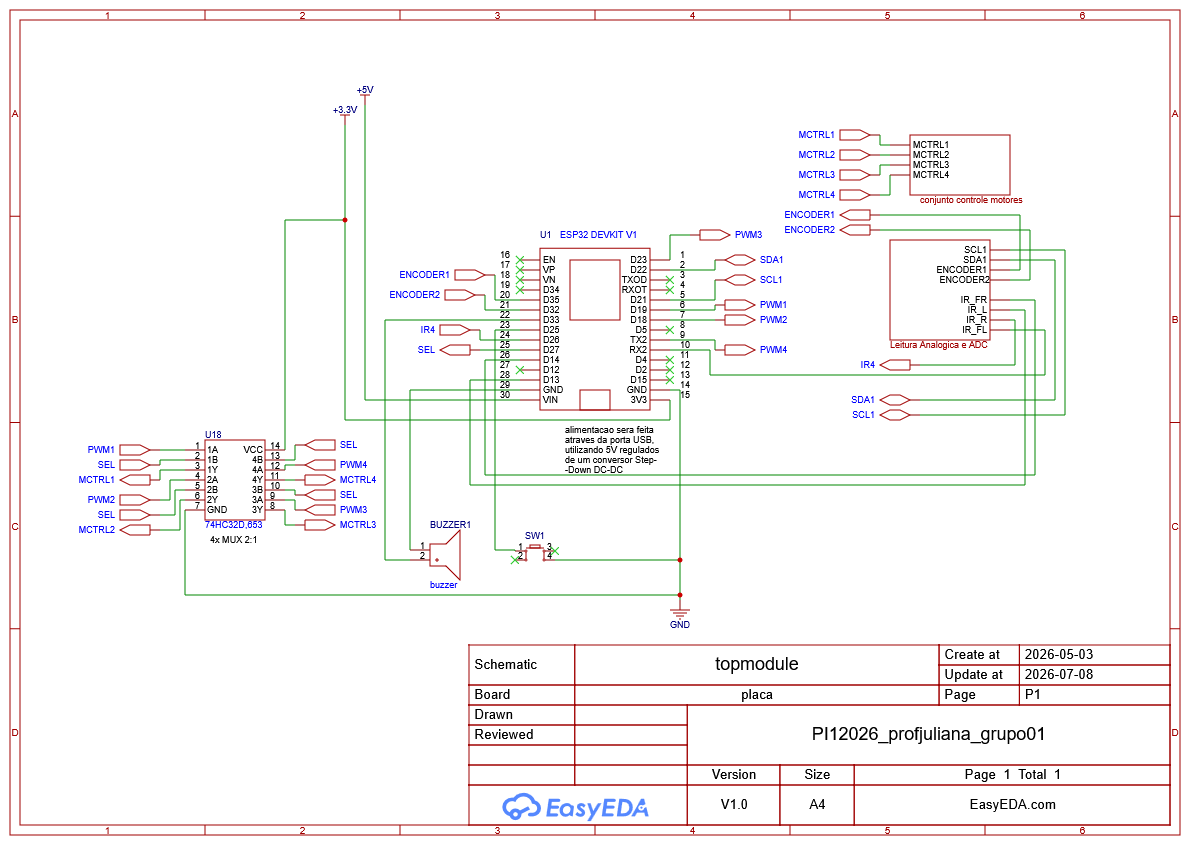
\includegraphics[width=0.5\linewidth]{figuras/SCH_topmodule_1-P1_2026-07-08.png}
    \caption{Representação da Ligação dos Componentes no Microcontrolador}
    \label{fig:esq_topmodule}
\end{figure}

\begin{figure}
    \centering
    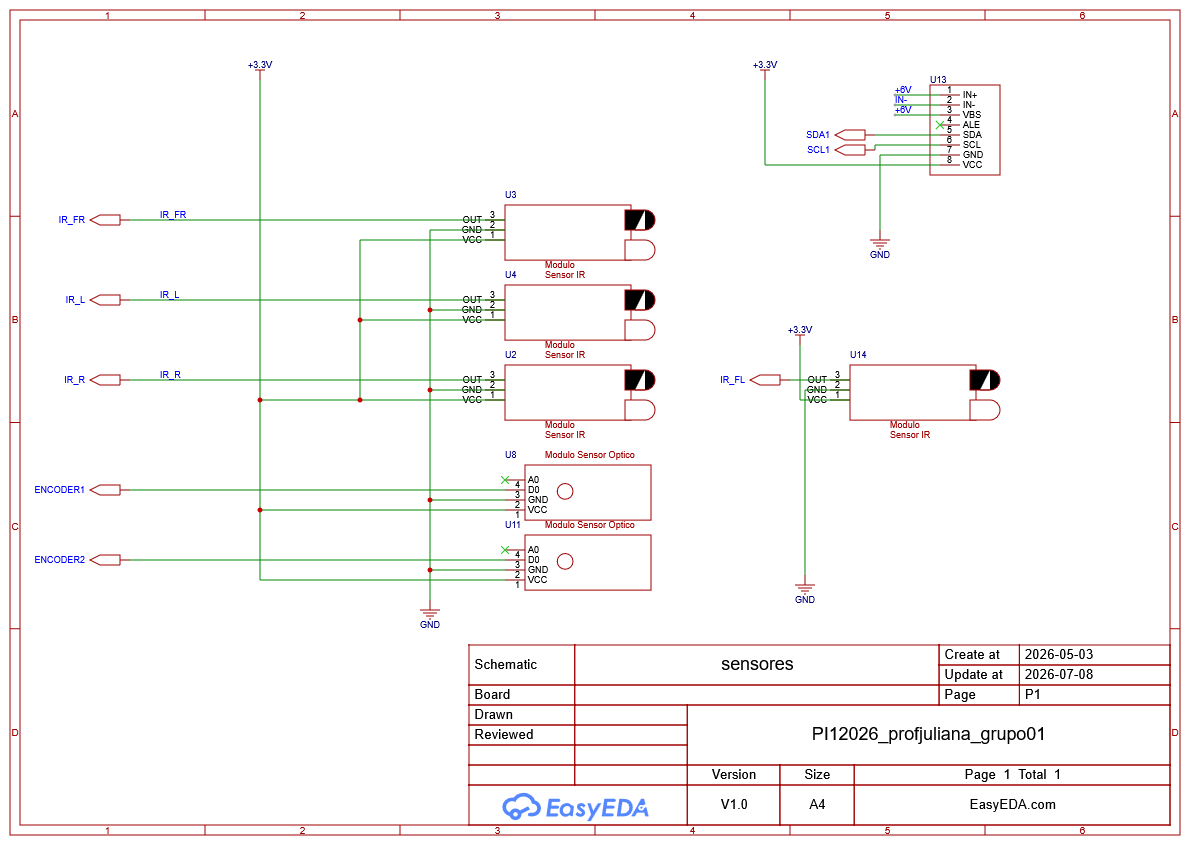
\includegraphics[width=0.5\linewidth]{figuras/SCH_sensores_1-P1_2026-07-08.png}
    \caption{Representação Esquemática dos Sensores}
    \label{fig:esq_sensores}
\end{figure}

\begin{figure}
    \centering
    
\includegraphics[width=0.5\linewidth]{figuras/SCH_motores_driver_1-P1_2026-07-08.png}
    \caption{Representação Esquemática do Driver e Motores}
    \label{fig:esq_motores}
\end{figure}

\begin{figure}
    \centering
    
\includegraphics[width=0.5\linewidth]{figuras/SCH_modulo_de_alimentacao_1-P1_2026-07-08.png}
    \caption{Representação Esquemática da Alimentação do \textit{Micromouse}}
    \label{fig:esq_alimentacao}
\end{figure}


\section{Justificativa da escolha dos componentes de \textit{hardware}}
\label{sec:justificativa-componentes}

Esta seção apresenta a justificativa técnica para a seleção de cada componente utilizado no projeto, considerando requisitos funcionais, disponibilidade, custo e compatibilidade com a arquitetura geral do sistema.

\subsection{ESP32-WROOM-32}

O microcontrolador ESP32-WROOM-32 foi selecionado por oferecer capacidade de processamento adequada para aplicações embarcadas, além de integração nativa com comunicação Wi-Fi e Bluetooth, possibilitando futura expansão do sistema. Segundo o trabalho apresentado no CONICT do IFSP, o ESP32 apresenta boa compatibilidade com sistemas robóticos devido à sua quantidade de portas de entrada e saída, baixo custo e facilidade de integração com sensores e atuadores. Além disso, sua operação em 3,3 V torna o componente compatível com módulos eletrônicos modernos utilizados no projeto.

Artigo base: \cite{oliveira2024_esp32_roboticar}

\subsection{Sensor Infravermelho (LM393)}

O sensor infravermelho LM393 foi selecionado para detecção de paredes e obstáculos do labirinto. Este módulo integra um LED infravermelho, um fototransistor e circuito de pré-processamento de sinais analógicos, oferecendo facilidade de implementação. O LM393 apresenta características técnicas adequadas para a aplicação: baixo consumo de energia (menos de 1 mA), ampla faixa de operação de tensão (2V a 36V), ângulo de difusão de 35° e alcance de 2 a 30 cm. Além disso, o sensor retorna sinais digitais ao microcontrolador, facilitando o processamento de dados. Por ser uma solução econômica e apresentar baixa complexidade de programação, o LM393 é apropriado para contextos educacionais e projetos com orçamento limitado.

Artigo base: \cite{lima2025_micromouse_lm393}

% \subsection{Bússola Magnetômetro (GY-271 HMC5883L)}

% O módulo GY-271 com magnet\^ometro HMC5883L foi escolhido por sua praticidade na identifica\c{c}\~ao da orienta\c{c}\~ao absoluta do rob\^o durante a navega\c{c}\~ao. No contexto do Micromouse, esse tipo de sensor pode ser usado como apoio para ajustar a virada do rob\^o ap\'os manobras de 90\textdegree\ ou 180\textdegree, ajudando a reduzir desvios acumulados e a confirmar se a mudan\c{c}a de dire\c{c}\~ao ocorreu de forma consistente com o comando enviado aos motores. Al\'em disso, por se tratar de um m\'odulo pequeno, de f\'acil integra\c{c}\~ao via I\textsuperscript{2}C e baixo consumo, sua utiliza\c{c}\~ao favorece a montagem do sistema embarcado sem aumento significativo de complexidade.

% Para garantir que a leitura n\~ao sofra interfer\^encia indevida dos motores, da ponte H ou de outros elementos do chassi, devem ser executados testes pr\'aticos com o rob\^o parado e tamb\'em em movimento. Os testes recomendados incluem: medi\c{c}\~ao da leitura de refer\^encia com o sistema desligado; compara\c{c}\~ao das leituras com motores desligados e ligados em diferentes rota\c{c}\~oes; valida\c{c}\~ao da varia\c{c}\~ao angular durante curvas conhecidas; e repeti\c{c}\~ao das medi\c{c}\~oes ap\'os altera\c{c}\~oes de posi\c{c}\~ao do sensor no chassi. Caso haja oscila\c{c}\~ao excessiva, o sensor deve ser reposicionado e a calibra\c{c}\~ao refeita at\'e que as leituras permane\c{c}am est\'aveis o suficiente para apoiar a corre\c{c}\~ao de orienta\c{c}\~ao do rob\^o.

% Fonte: \cite{eletrogate_bussola}

\subsection{Driver Ponte H (DRV8833)}

O driver DRV8833 foi escolhido por permitir o controle independente de dois motores DC, oferecendo controle de velocidade e direção através de PWM. O componente apresenta baixo consumo energético, suporte a tensões compatíveis com o ESP32 e mecanismos internos de proteção contra sobrecorrente e superaquecimento, aumentando a segurança do sistema. Conforme descrito na documentação técnica da Texas Instruments e em aplicações embarcadas similares, o DRV8833 é amplamente utilizado em robôs móveis compactos devido à sua eficiência energética e tamanho reduzido.

Artigo base: \cite{oliveira2024_esp32_roboticar}

\subsection{Regulador de Tensão Step-Down (LM2596)}

O módulo regulador LM2596 foi adotado para garantir estabilidade na alimentação elétrica do sistema, realizando a conversão eficiente da tensão fornecida pela bateria para níveis adequados aos demais componentes eletrônicos. De acordo com o artigo do CONICT do IFSP, o LM2596 é amplamente empregado em sistemas embarcados por apresentar boa eficiência energética, baixo custo e facilidade de integração. Sua utilização contribui para a proteção dos circuitos e para o funcionamento estável do microcontrolador e dos sensores.

Artigo base: \cite{oliveira2024_esp32_roboticar}

\subsection{Chave Óptica para Encoder (MOCH22A)}

O sensor óptico MOCH22A foi escolhido para a detecção de velocidade e posição das rodas, pois permite gerar pulsos a partir da passagem das marcas do disco encoder acoplado ao eixo do motor. A partir da contagem desses pulsos em intervalos de tempo conhecidos, o sistema consegue estimar a rotação do motor e, com isso, também estimar variações de velocidade e rotação do rob\^o durante manobras e deslocamentos no labirinto. Com esses dados, se faz uso de equações de movimento conhecidas para determinar a posição relativa do robô e seu deslocamento (CORKE, 2011). Esse tipo de realimenta\c{c}\~ao \^e importante para o controle mais preciso da locomoc\~ao, principalmente em trajet\'orias curtas e corre\c{c}\~oes finas de movimento.

Embora a refer\^encia base utilize Arduino, o princ\'ipio de funcionamento \^e diretamente adapt\'avel ao ESP32, que tamb\'em possui suporte a interrup\c{c}\~oes e opera\c{c}\~ao adequada com leitura digital de pulsos. Dessa forma, o MOCH22A contribui para o sistema embarcado ao fornecer feedback confi\'avel de rota\c{c}\~ao, com baixo custo, montagem simples e boa integra\c{c}\~ao com a l\'ogica de controle do motor.

Fontes:~\cite{makerhero_moch22a}, \cite{petercorke}

\subsection{Sensor de Potência (INA226)}

O sensor de potência INA226 foi escolhido para substituir os sensores individuais de tensão e corrente e realizar o monitoramento do consumo energético com mais precisão e economia de espaço. Este sensor realiza suas leituras e as armazena em registradores próprios no chip do sensor, bastando apenas selecionar o registrador da grandeza desejada para obter a sua leitura. Isso é um fator decisivo para a gestão de processamento do projeto. Além disso, o sensor trabalha com comunicação I²C, possibilitando comunicação rápida e robusta com a ESP32.

\subsection{Porta Lógica 74HC32 (OU lógico)}

Este Circuito Integrado foi escolhido com a finalidade de realizar a multiplexação das entradas do driver DRV8833, visto que, para obter o freio ativo deste, era necessário que as entradas fossem 1 lógico (ou "high"). Assim, multiplexando as entradas da ponte H, evita-se que os GPIOs da ESP tenham de ser reconfigurados frequentemente entre GPIOs PWM e GPIOs comuns, economizando processamento e linhas de código desnecessárias. 

\subsection{Buzzer Passivo}

O buzzer passivo foi escolhido para a sinalização sonora por apresentar menor dimens\~ao e peso em rela\c{c}\~ao ao buzzer ativo, o que contribui para a redu\c{c}\~ao do volume e da massa total do sistema. Al\'em disso, seu uso permite um projeto de acionamento mais simples do ponto de vista de integra\c{c}\~ao ao conjunto eletr\'onico, e seu custo inferior em compara\c{c}\~ao ao buzzer ativo torna a solu\c{c}\~ao mais econ\^omica para o projeto.

Fonte: \cite{makerhero_buzzer}
